\documentclass{beamer}
\usepackage{tcolorbox}
\usepackage{graphicx}
\usepackage{amsmath}
\usepackage[labelformat=empty]{caption}

\usepackage{hyperref}
\hypersetup{
    colorlinks=true,
    linkcolor=blue,
    filecolor=magenta,      
    urlcolor=cyan,
}

\usepackage{tikz}
\def\checkmark{\tikz\fill[scale=0.4](0,.35) -- (.25,0) -- (1,.7) -- (.25,.15) -- cycle;} 


%\beamerdefaultoverlayspecification{<+->}
\newcommand{\data}{\mathcal{D}}

\DeclareMathOperator*{\argmin}{arg\,min}

\newcommand\Item[1][]{%
	\ifx\relax#1\relax  \item \else \item[#1] \fi
	\abovedisplayskip=0pt\abovedisplayshortskip=0pt~\vspace*{-\baselineskip}}
	


\usetheme{metropolis}           % Use metropolis theme


\title{Accuracy metrics, Classification, Regression}
\date{\today}
\author{Nipun Batra}
\institute{IIT Gandhinagar}
\begin{document}
  \maketitle
  
  
  
\section{Classification}

\begin{frame}{Feature Table}
\begin{figure}[htp]
    \centering
    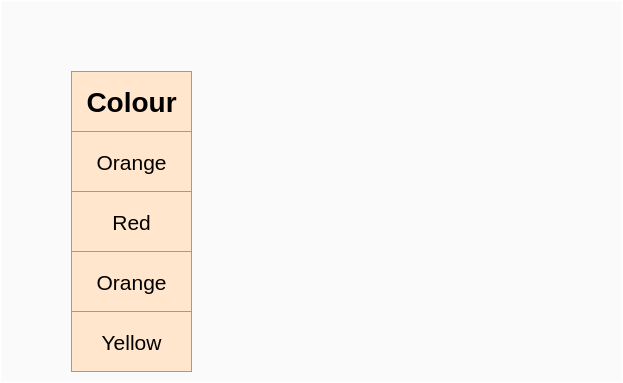
\includegraphics[width=0.7\linewidth]{accuracy/ml_2_accuracy_table_1.png}
\end{figure}
\end{frame}

\begin{frame}{Feature Table}
\begin{figure}[htp]
    \centering
    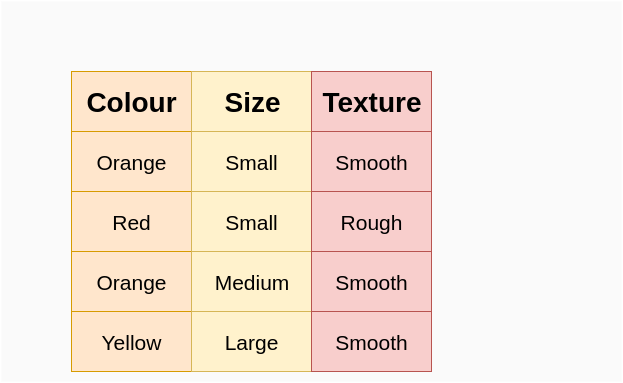
\includegraphics[width=0.7\linewidth]{accuracy/ml_2_accuracy_table_2.png}
\end{figure}
\end{frame}

\begin{frame}{Feature Table}
\begin{figure}[htp]
    \centering
    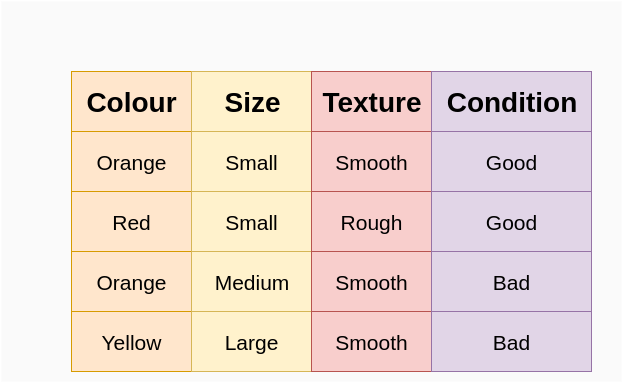
\includegraphics[width=0.7\linewidth]{accuracy/ml_2_accuracy_table_3.png}
\end{figure}
\end{frame}

\begin{frame}{Feature Table}
\begin{figure}[htp]
    \centering
    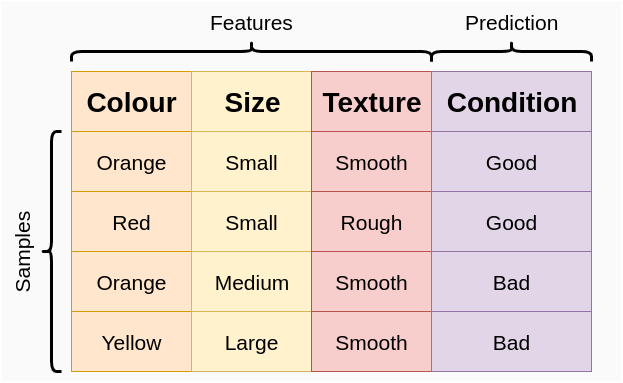
\includegraphics[width=0.7\linewidth]{accuracy/ml_2_accuracy_table_4.png}
    \caption{Training Set for Supervised Learning}
\end{figure}
\end{frame}

\begin{frame}{Feature Table}
\begin{figure}[htp]
    \centering
    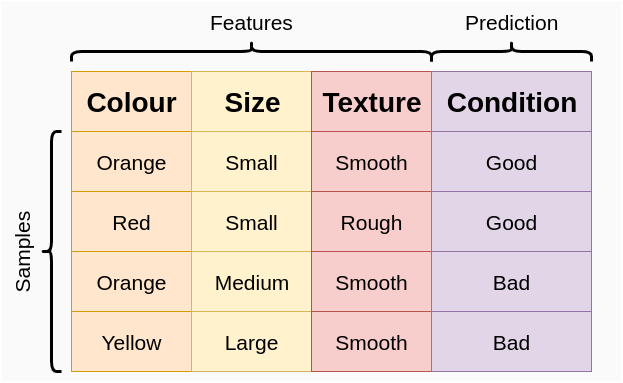
\includegraphics[width=0.7\linewidth]{accuracy/ml_2_accuracy_table_4.png}
\end{figure}
We hope to learn $f$, where:
\begin{tcolorbox}
\begin{center}
$\texttt{Condition} = f(\texttt{colour, size, texture})$
\end{center}
\end{tcolorbox}
\end{frame}

\begin{frame}{Classification}
\begin{figure}[htp]
    \centering
    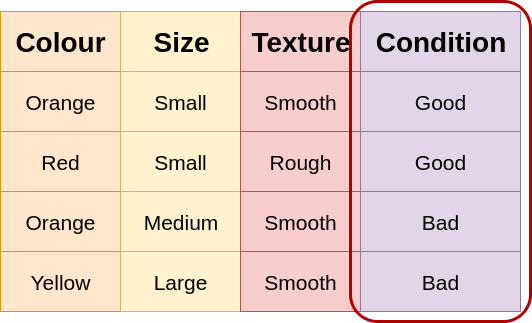
\includegraphics[width=0.7\linewidth]{accuracy/ml_2_accuracy_table_5.png}
\end{figure}

\begin{center}
Condition here is discrete $\rightarrow$ \textbf{Classification}
\end{center}

\end{frame}

\begin{frame}{Accuracy Metrics}
$$\bordermatrix{&\texttt{Prediction}\;(\hat{y})\cr
                &\texttt{Good}\cr
                &\texttt{Good}\cr
                &\texttt{Good}\cr
                &\texttt{Good}\cr
                &\texttt{Bad}}
                \qquad \qquad
   \bordermatrix{&\texttt{Ground Truth}\cr
                &\texttt{Good}\cr
                &\texttt{Good}\cr
                &\texttt{Bad}\cr
                &\texttt{Bad}\cr
                &\texttt{Bad}}
$$

\vspace{1cm}

\begin{tabular}{ll}
Ground Truth: & From the actual training set \\ 
Prediction: & Made by the model \\ 
\end{tabular}

\end{frame}

\begin{frame}{Accuracy Metrics: Accuracy}
$$
\bordermatrix{&\texttt{Prediction}\;(\hat{y})\cr
               \checkmark&\texttt{Good}\cr
               \checkmark&\texttt{Good}\cr
                &\texttt{Good}\cr
                &\texttt{Good}\cr
               \checkmark&\texttt{Bad}}
\qquad \qquad
\bordermatrix{&\texttt{Ground Truth}\cr
                &\texttt{Good}\cr
                &\texttt{Good}\cr
                &\texttt{Bad}\cr
                &\texttt{Bad}\cr
                &\texttt{Bad}}
$$

\begin{align*}
\texttt{Accuracy} &= \frac{||y = \hat{y}||}{||y||} \\
&= \frac{3}{5} = 0.6
\end{align*}

\end{frame}

\begin{frame}{Types of Data: Imbalanced Classes}
\[
  \begin{array}{@{} c @{}}
    \begin{array}{@{} r @{}}
      \text{1 sample}~\{\hspace{\nulldelimiterspace} \\
      \text{100 samples}~\left\{\begin{array}{@{}c@{}}\null\\\null\\\null\\\null\end{array}\right.
    \end{array}
    \left (
      \begin{array}{ *{1}{c} }
        \texttt{Bad}  \\
        \texttt{Good}  \\
        \texttt{Good}  \\
        \ldots  \\
        \texttt{Good}  \\
      \end{array}
    \right ) \\
    \mathstrut
  \end{array}
  \quad \quad \quad
  \text{Imbalanced Classes}
\]

\pause

Cases for this:
\begin{itemize}%[<+->]
\item Cancer Screening
\item Planet Detection
\end{itemize}

\end{frame}

\begin{frame}{Accuracy Metrics: Precision}
$$
\bordermatrix{&\texttt{Prediction}\;(\hat{y})\cr
               \rightarrow\checkmark&\texttt{Good}\cr
               \rightarrow\checkmark&\texttt{Good}\cr
                \rightarrow&\texttt{Good}\cr
                \rightarrow&\texttt{Good}\cr
               &\texttt{Bad}}
\qquad \qquad
\bordermatrix{&\texttt{Ground Truth}\cr
                &\texttt{Good}\cr
                &\texttt{Good}\cr
                &\texttt{Bad}\cr
                &\texttt{Bad}\cr
                &\texttt{Good}}
$$

\begin{align*}
\texttt{Accuracy} &= \frac{||y = \hat{y} = \texttt{Good}||}{||\hat{y} = \texttt{Good}||} = \frac{2}{4} = 0.5
\end{align*}

``the fraction of relevant instances among the retrieved instances''

\end{frame}

\begin{frame}{Accuracy Metrics: Recall}
$$
\bordermatrix{&\texttt{Prediction}\;(\hat{y})\cr
               \rightarrow\checkmark&\texttt{Good}\cr
               \rightarrow\checkmark&\texttt{Good}\cr
                &\texttt{Good}\cr
                &\texttt{Good}\cr
               \rightarrow&\texttt{Bad}}
\qquad \qquad
\bordermatrix{&\texttt{Ground Truth}\cr
                &\texttt{Good}\cr
                &\texttt{Good}\cr
                &\texttt{Bad}\cr
                &\texttt{Bad}\cr
                &\texttt{Good}}
$$

\begin{align*}
\texttt{Accuracy} &= \frac{||y = \hat{y} = \texttt{Good}||}{||y = \texttt{Good}||} = \frac{2}{3} = 0.67
\end{align*}

``the fraction of the total amount of relevant instances that were actually retrieved''

\end{frame}

\begin{frame}{Types of Data: Imbalanced Classes}
Given predictions of weather a tissue is cancerous or not ($n = 100$).
$$
\bordermatrix{&\texttt{Prediction}\;(\hat{y})\cr
               \rightarrow&\texttt{No}\cr
               &\texttt{Yes}\cr
                &\texttt{Yes}\cr
                &\ldots\cr
               &\texttt{Yes}}
\qquad \qquad
\bordermatrix{&\texttt{Ground Truth}\cr
                &\texttt{Yes}\cr
                &\texttt{Yes}\cr
                &\ldots\cr
                &\texttt{Yes}\cr
                \rightarrow&\texttt{No}}
$$

\begin{align*}
\texttt{Accuracy} = \frac{98}{100} = 0.98 \qquad \qquad \qquad
\texttt{Recall} &= \frac{0}{99} = 0 \\
\texttt{Precision} &= \frac{0}{99} = 0
\end{align*}


\end{frame}

\begin{frame}{Accuracy Metrics: Confusion Matrix}
For the same data
$$
\bordermatrix{&\texttt{G.T. Positive}&\texttt{G.T. Negative}\cr
               \texttt{Pred Positive}&0&1\cr
               \texttt{Pred Positive}&1&98}
$$
$$
\bordermatrix{&\texttt{G.T. Positive}&\texttt{G.T. Negative}\cr
               \texttt{Pred Positive}&\texttt{True Positive}&\texttt{False Positive}\cr
               \texttt{Pred Positive}&\texttt{True Negative}&\texttt{False Negative}}
$$


\begin{align*}
\texttt{Recall} = \frac{\texttt{T.P}}{\texttt{T.P + F.P}} \qquad \qquad 
\texttt{Precision} = \frac{\texttt{T.P}}{\texttt{T.P + F.N}}
\end{align*}
\end{frame}

\begin{frame}{Accuracy Metrics: F-Score}
For the same data
$$
\bordermatrix{&\texttt{G.T. Positive}&\texttt{G.T. Negative}\cr
               \texttt{Pred Positive}&\texttt{True Positive}&\texttt{False Positive}\cr
               \texttt{Pred Positive}&\texttt{True Negative}&\texttt{False Negative}}
$$

$$
\texttt{F-Score} = \frac{2\times\texttt{Precision}\times\texttt{Recall}}{\texttt{Precision} + \texttt{Recall}}
$$


\end{frame}


\begin{frame}{Accuracy Metrics: Matthew's Correlation Coefficient}
For the same data
$$
\bordermatrix{&\texttt{G.T. Positive}&\texttt{G.T. Negative}\cr
               \texttt{Pred Positive}&\texttt{True Positive}&\texttt{False Positive}\cr
               \texttt{Pred Positive}&\texttt{True Negative}&\texttt{False Negative}}
$$

\texttt{Matthew's Correlation Coefficient =}
$$
\frac{\texttt{TP $\times$ TN} - \texttt{FP $\times$ FN}}{\sqrt{\texttt{(TP + FP)(TP + FN)(TN + FP)(TN + FN)}}}
$$
\end{frame}

\begin{frame}{Accuracy Metrics: Example}
For the same data
$$
\bordermatrix{&\texttt{G.T. Positive}&\texttt{G.T. Negative}\cr
               \texttt{Pred Positive}&90&4\cr
               \texttt{Pred Positive}&1&1}
$$

Precision = ?  \\
Recall = ?\\
F-Score = ?\\
Matthew's Coeff. = ?\\
\end{frame}

\begin{frame}{Accuracy Metrics: Answer}
For the same data
$$
\bordermatrix{&\texttt{G.T. Positive}&\texttt{G.T. Negative}\cr
               \texttt{Pred Positive}&90&4\cr
               \texttt{Pred Positive}&1&1}
$$

Precision = $\frac{90}{94}$ \\
Recall = $\frac{90}{91}$ \\
F-Score = 0.9524 \\
Matthew's Coeff. = 0.14
\end{frame}


\section{Regression}

\begin{frame}{Regression Examples}
\begin{figure}[htp]
    \centering
    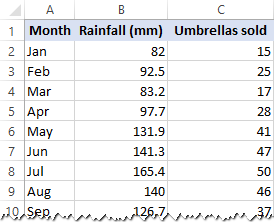
\includegraphics[width=0.7\linewidth]{accuracy/reg1.png}
\end{figure}

\pause

Regression involves continuous data.
\end{frame}

\begin{frame}{Accuracy Metrics: MSE \& MAE}
$$
\bordermatrix{&\texttt{Prediction}\;(\hat{y})\cr
               &10\cr
               &20\cr
                &30\cr
                &40\cr
               &50}
\qquad \qquad
\bordermatrix{&\texttt{Ground Truth}\cr
               &20\cr
               &30\cr
                &40\cr
                &50\cr
               &60}
$$

\begin{align*}
\texttt{Mean Square Error (MSE)} &=  \frac{\sum_{}^{}(\hat{y}-y)^2}{N} \\ 
\texttt{Root Mean Square Error (RMSE)} &=  \sqrt{\texttt{MSE}}
\end{align*}

\end{frame}

\begin{frame}{Accuracy Metrics: MAE \& ME}
$$
\bordermatrix{&\texttt{Prediction}\;(\hat{y})\cr
               &10\cr
               &20\cr
                &30\cr
                &40\cr
               &50}
\qquad \qquad
\bordermatrix{&\texttt{Ground Truth}\cr
               &20\cr
               &30\cr
                &40\cr
                &50\cr
               &60}
$$

\begin{align*}
\texttt{Mean Absolute Error (MAE)} &=  \frac{\sum_{}^{}|\hat{y}-y|}{N} \\ 
\texttt{Mean Error} &=  \frac{\sum_{}^{}\hat{y}-y}{N}
\end{align*}

\end{frame}

\begin{frame}{The Importance of Plotting}
\begin{figure}[htp]
    \centering
    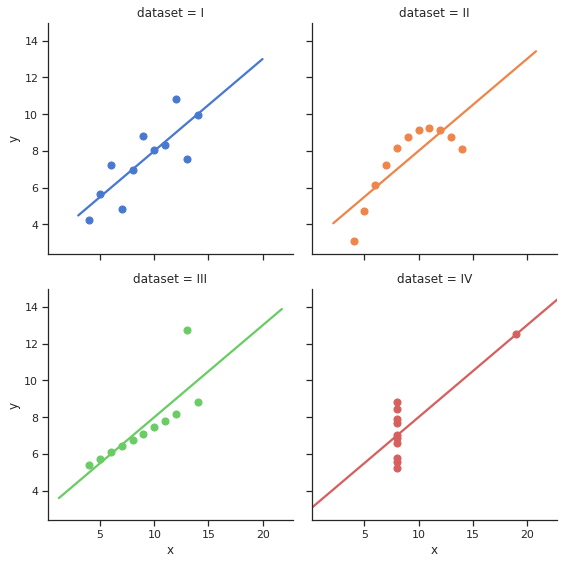
\includegraphics[width=0.6\linewidth]{accuracy/ans1.png}
    \caption{Anscombe’s Quartet}
\end{figure}
\end{frame}

\begin{frame}{The Importance of Plotting}
\begin{tabular}{|c|c|c|}
\hline 
Property & Value & Accross datasets \\ 
\hline 
mean(X) & 9 & exact \\ 
mean(Y) & 7.5 & upto 3 decimal places \\ 
Linear regression line & 	y = 3.00 + 0.500x & upto 2 decimal places \\ 
\hline 
\end{tabular} 

Try to play with the \href{https://colab.research.google.com/drive/12Rrh7sf_lR-WUd4nYciOAKiil5kqWPAq}{colab link} to see how similar the metrics like variance and correlation are.

\end{frame}

\end{document}